\cleardoublepage

\section{绪论}

\subsection{背景}

\subsubsection{GPU的高速发展}

GPU是图形处理器单元(Graphics Processing Unit)的缩写。GPU自20世纪90年代中期诞生以来,已经从最初的简单图形渲染设备发展成为现代计算中不可或缺的高性能并行处理器。最初的GPU主要负责处理2D图形,随着技术的进步,现代GPU不仅能够处理复杂的3D图形,还能够执行通用的并行计算任务。这一转变始于NVIDIA推出CUDA平台和ATI(现为AMD)推出Stream架构,它们使得GPU能够运行非图形相关的并行计算程序,从而开启了GPU通用计算的新时代。

消费级的 GPU 通常有上千个核心——特别适合处理大型数据集,因此,GPU在数据密集,计算密集,高性能计算的领域大放异彩。在消费电子领域,GPU为游戏,视频编辑和高清视频播放等提供了图形处理能力;在专业图形设计领域,GPU为汽车,航空,建筑和娱乐等行业提供了3D建模和渲染能力;在科研领域,GPU能够加速物理模拟,生物信息学和气候模型等领域的数值计算;在数据中心和云计算领域,GPU在加速数据库处理、加密计算和机器学习任务中发挥着重要作用;在自动驾驶和机器人技术方面,GPU用于处理传感器数据和执行复杂的决策算法;在最近新兴的人工智能领域,大批量的GPU用于神经网络的训练和推理。

可以肯定的说,目前世界上主流的高新技术产业的发展都难以离开GPU的支持,GPU的短缺甚至会阻塞如人工智能等领域的研究和发展。

\subsubsection{GPU的产业竞争}

自GPU问世起,GPU产业的主导权就一直掌握在NVDIA公司中,除此之外只有Intel,AMD等少数科技公司在GPU市场上留有一席之地,可以说,GPU市场是由少数公司垄断的,是由美国主导的。


目前人工智能,自动驾驶等前沿科技的高速发展, 以及高性能GPU工艺特性导致的产能低下使得全球范围内出现GPU的短缺,尤其是高性能GPU的短缺,同时也愈加凸显GPU市场份额的重要性。

为了取得深度学习和人工智能等高新产业的主导权,我国势必要建立本土GPU产业,特别是高性能国产GPU企业,解决我国目前如NVDIA 40系列,A系列芯片等高性能GPU短缺的现状。因而对高性能GPU的研究应当是各企业,研究所的攻关重点。

\subsubsection{GPU微架构}

要想提升国产GPU的性能,首先要从GPU的架构入手,以下是现代GPU的核心组成部分和概念:
\begin{enumerate}
    \item 核心(Core):GPU的核心是执行图形和计算任务的处理器。现代GPU通常拥有成百上千个核心,这些核心可以并行处理大量的数据。
    \item 流处理器(Streaming Processor):在NVIDIA的架构中,核心通常被称为流处理器(CUDA核心)。这些核心专门设计用于执行图形和并行计算任务。
    \item 纹理单元(Texture Unit):纹理单元负责将纹理映射到3D模型上。在现代GPU中,纹理单元的数量通常与核心数量成正比。
    \item 光栅化器(Rasterizer):光栅化器负责将3D模型的顶点转换为2D屏幕上的像素。
    \item 几何着色器(Geometry Shader):几何着色器可以创建新的顶点和几何图形,这在复杂的3D场景渲染中非常有用。
    \item 张量核心(Tensor Core):在NVIDIA的某些高端GPU中,张量核心被设计用于深度学习任务,可以极大提高AI计算的效率。
    \item 内存接口(Memory Interface):GPU的内存接口决定了它与外部内存(如RAM)的交互速度。这包括了内存带宽和内存类型(如GDDR5、GDDR6等)。
    \item 缓存(Cache):缓存是一种快速的内存,用于存储GPU频繁访问的数据,以减少对主内存的访问次数。
    \item 虚拟内存(Virtual Memory):一些GPU支持虚拟内存,允许它们使用系统RAM作为额外的图形内存。
    \item 功耗和热设计功率(TDP):微架构设计还需要考虑GPU的功耗和散热问题,以确保设备在安全的温度下运行。
    \item 统一着色器架构(Unified Shader Architecture):一些GPU设计采用了统一着色器架构,这意味着不同类型的着色器(如顶点着色器、像素着色器等)可以共享核心资源。
    \item 多线程和多实例(Multi-Threading and Multi-Instancing):现代GPU支持多线程和多实例技术,允许单个核心同时处理多个任务。
    \item 异步计算(Asynchronous Compute):异步计算允许GPU在渲染的同时执行其他计算任务,提高了整体的计算效率。
    \item 硬件虚拟化(Hardware Virtualization):一些GPU支持硬件虚拟化,允许在单个物理GPU上模拟多个GPU。
    \item 错误校正码(ECC):在某些专业级GPU中,错误校正码用于检测和纠正内存中的错误,这对于需要高可靠性的应用(如科学计算)非常重要。
\end{enumerate}

了解GPU微架构对于优化图形和计算应用程序的性能至关重要。不同的GPU制造商(如NVIDIA、AMD、Intel等)都有自己的微架构设计,每种设计都有其独特的特点和优势。我们国产GPU要想进军高性能GPU领域,一定要着手研发自己的微架构设计。其中,优化光栅化模块是提升GPU图形处理能力是重中之重,本课题将从GPU中的光栅化器入手,从光栅化模块的角度来提升GPU的图形处理能力。


\subsubsection{GPU中的光栅化微架构}
光栅化器(Rasterizer)是GPU中的一个关键组件,它负责将3D图形的顶点数据转换成2D屏幕上的像素点,从而生成最终的图像。这个过程被称为光栅化(Rasterization)。以下是光栅化器的一些关键功能和概念:

\begin{enumerate}
    \item 顶点处理:在光栅化之前,GPU会执行顶点处理,计算每个顶点的位置、颜色、纹理坐标等属性。这些顶点数据通常由应用程序提供,并在GPU的顶点着色器中进行处理。
    \item 三角形设置:顶点处理完成后,GPU会将相邻的三个顶点组成一个三角形。三角形是3D图形中最基本的几何形状,所有复杂的3D模型都可以分解成许多小的三角形。
    \item 三角形裁剪:在光栅化之前,GPU会进行三角形裁剪,将三角形与视口(View Frustum)相交的部分裁剪掉。视口是一个金字塔形的区域,代表摄像机的视野范围。裁剪可以减少不必要的计算,提高渲染效率。
    \item 三角形遍历:光栅化器会遍历三角形内部的像素点,确定哪些像素点属于该三角形。这个过程称为三角形遍历(Triangle Traversal)。光栅化器会使用各种算法来高效地遍历像素点,如扫描线算法、边缘生长算法等。
    \item 像素着色器执行:对于每个遍历到的像素点,光栅化器会执行像素着色器(Pixel Shader)来计算该像素的颜色值。像素着色器可以访问三角形的顶点数据,并根据顶点属性和纹理等信息计算出像素的颜色。
    \item 深度测试和模板测试:在像素着色器执行完成后,光栅化器会进行深度测试(Depth Test)和模板测试(Stencil Test)。深度测试会根据像素的深度值(Z值)决定该像素是否可见,模板测试会根据模板缓冲区(Stencil Buffer)的值决定该像素是否应该被渲染。
    \item 混合和反走样:对于通过深度和模板测试的像素,光栅化器会执行混合(Blending)和反走样(Anti-Aliasing)操作。混合会根据像素的颜色和混合状态将新像素与帧缓冲区(Frame Buffer)中的现有像素进行混合。反走样可以平滑锯齿状的边缘,提高图像质量。
    \item 多采样抗锯齿(MSAA):为了提高反走样的质量,一些GPU支持多采样抗锯齿。MSAA会在每个像素点上存储多个样本,然后对这些样本进行平均,以减少走样伪影。
    \item 帧缓冲区写入:最后,光栅化器会将计算得到的颜色值写入帧缓冲区。帧缓冲区是GPU的内存区域,用于存储最终渲染的图像。
\end{enumerate}
\begin{figure}
    \centering

    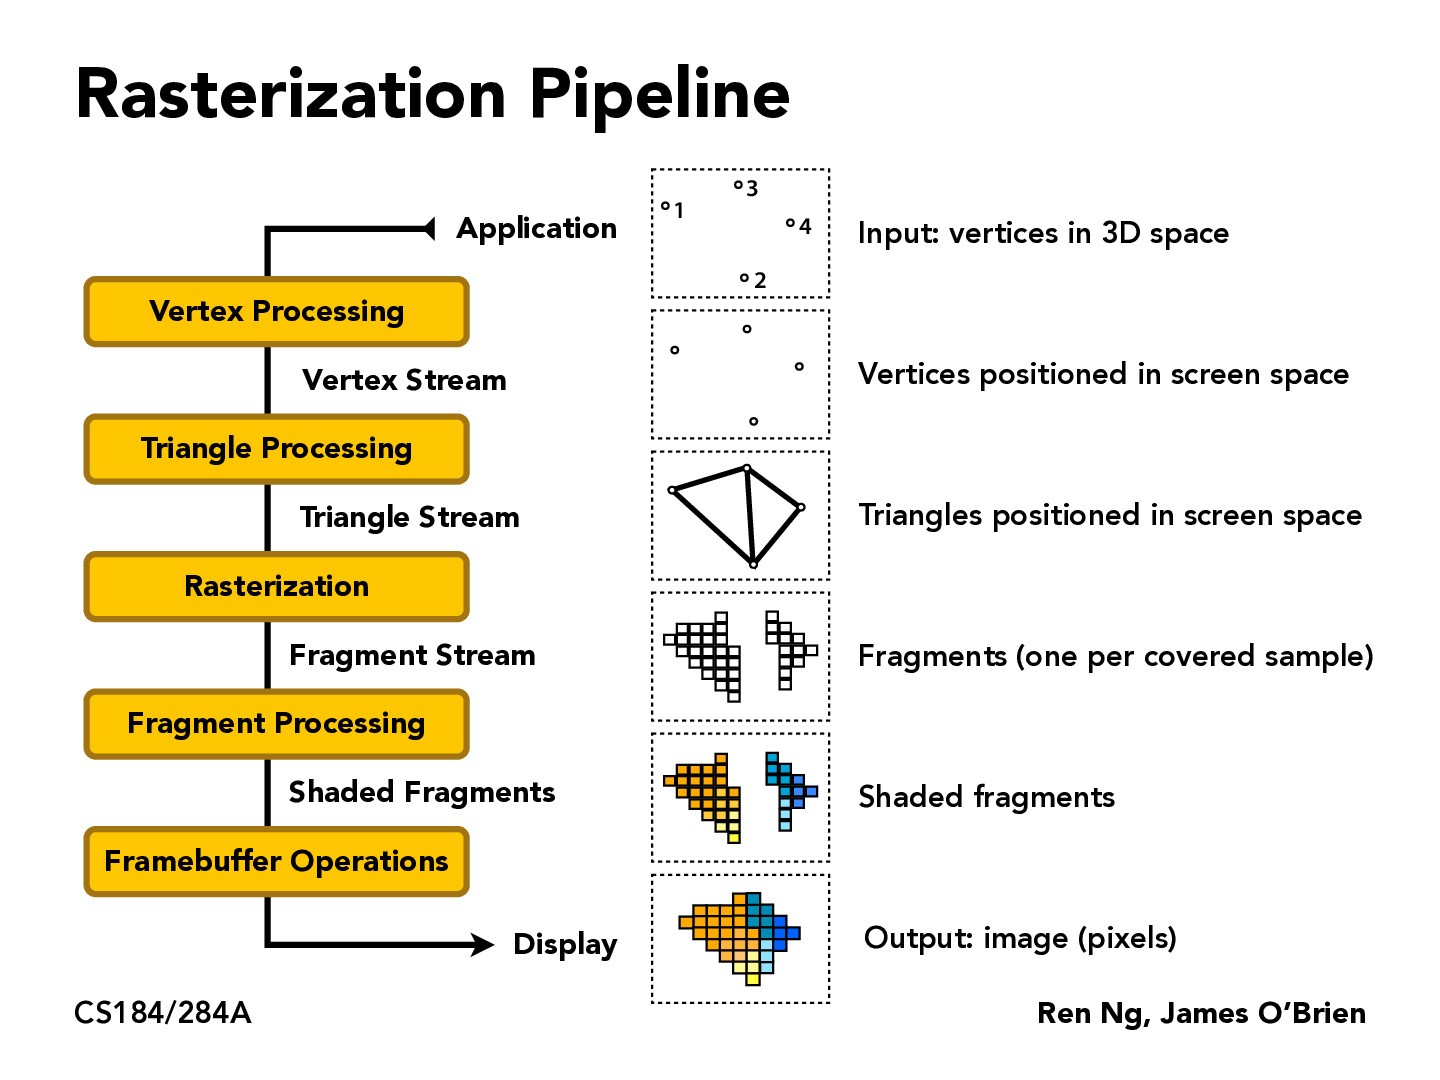
\includegraphics[width = .5\textwidth]{figure/rasterization_pipeline.jpeg.jpg}
    \caption{光栅化流水线}
    \label{fig:rast pipeline}
\end{figure}
光栅化是3D图形渲染流水线中非常关键的一步,它直接影响到最终图像的质量。优化光栅化过程可以显著提高渲染效率和图像质量。不同的GPU架构和渲染API(如DirectX、OpenGL、Vulkan等)在光栅化器的实现上可能有所不同,但基本原理是相似的。

在光栅化模块中,显然三角形遍历是整个光栅化流水线的性能瓶颈, 本课题从这一点出发,设计更具有并行性的点在三角形内测试算法(即判断屏幕空间内的一点是否在给定的三角形中)。


\subsubsection{本文的研究内容与意义}
本文的研究内容是从国产GPU的光栅化器微架构入手,设计适用于光栅化器中的高并行性的点在三角形测试算法,用来提升国产GPU中光栅化器三角形遍历的效率,进而提升国产GPU的光栅化性能。

本文的研究与国产GPU厂商合作,对国产GPU高性能架构做出了一定的探索,为国产高性能GPU技术研发的自主化做出了一定的贡献,助力了国产GPU的生态建设。

\subsubsection{本文的架构}

本文将分六个章节展开叙述:

\begin{itemize}
    \item 第一章为绪论,主要讲述了本文的工作背景,阐述了本文的研究内容在国产高性能GPU发展的进程中起到的积极作用。
    \item 第二章为技术路线,主要讲述了本文的研究的技术基础,参考的已有算法。
    \item 第三章为系统设计,讲述了本文的原型系统的设计细节,和算法的运行过程。
    \item 第四章为系统的并行性分析和优化,对第三章中提出的原型系统做了并行性的分析,并提出了并行优化策略。
    \item 第五章为系统的测试结果与分析,第五章中队第四章提出优化并行系统做了正确性验证,和不同参数下的性能测试,并通过分析对并行系统做了进一步的性能调优。
    \item 第六章是本文的总结,总结了本文的工作内容,指出了本文的不足以及未来可以改进的方向。
\end{itemize}


